\documentclass[12pt, 
    twoside=false, 
    bibliography=totoc, 
    numbers=endperiod, 
    headings=normal, 
    toc=chapterentrydotfill
    ]{scrbook}
\usepackage[utf8]{inputenc}
\usepackage[ngerman]{babel}
\usepackage{blindtext}
\usepackage{csquotes}
\usepackage{booktabs}
\usepackage{setspace}
\usepackage{mathpazo}
\usepackage{graphicx}
\usepackage[
  	pdfstartview=FitH,   
  	pdffitwindow=true,
  	colorlinks,
  	linkcolor=black,
  	anchorcolor=black,
  	citecolor=black,
  	urlcolor=black
  	]{hyperref}
\usepackage[labelfont=bf]{caption}
\usepackage{float}
\usepackage[
    backend=biber, 
    style=authoryear-ibid, 
    eprint=false,
    url=false,
    doi=false,
    isbn=false
    ]{biblatex}
\addbibresource{Bib.bib}

\setkomafont{sectioning}{\normalcolor\bfseries}
\renewcommand*{\chapterheadstartvskip}{\vspace*{-\topskip}}
\KOMAoptions{headsepline = true}

\begin{document}

\begin{titlepage}
    \begin{minipage}[t]{0.6\textwidth}
    \flushleft 
    Universität Hamburg \\
    Fachbereich: Sozialwissenschaften \\
    Fachgebiet: Politikwissenschaft \\
    Seminar: Forschungsseminar Vergleichende und Regionalstudien \\ 
    Dozenten: Prof. Kai-Uwe Schnapp \\
    PD Dr. Falk Daviter \\
    Wintersemester 2018/19 \\
    \end{minipage}
    \hfill
    \begin{minipage}[t][1.7cm][b]{0.35\textwidth}
    
\includegraphics[width=\textwidth]{images/UHH-Logo_2010_Farbe_CMYK.pdf}
    \end{minipage}
    
    \vspace*{\fill}
    \begin{center}
	\vspace{1cm}\noindent {\textbf{Projektarbeit}} \vspace{0.2cm} \\
	\textbf{\Large Geschlechterunterschiede} \\
	\textbf{WIP} \\
	\vspace{0.2cm}
	30.03.2019
	\end{center}
    \vspace*{\fill}
	
	\begin{minipage}[t]{0.48\textwidth}
    \flushleft 
    Gina-Gabriela Görner \\
    Matrikelnummer: XXX \\
    XXX \vspace{0.1cm} \\ 
	XXX \vspace{0.1cm}  \\
	E-Mail: XXX \\ 
    \end{minipage}
    \begin{minipage}[t]{0.48\textwidth}
	\flushleft
	Josef Holnburger \\
	Matrikelnummer: XXX \\
	XXX \vspace{0.1cm} \\
	XXX \vspace{0.1cm} \\
	E-Mail: josef@holnburger.com \\
    \end{minipage}

\end{titlepage}

\frontmatter

\tableofcontents

\listoffigures
\addcontentsline{toc}{chapter}{\listfigurename}
\vspace*{24pt}
{\let\clearpage\relax \listoftables}	
\addcontentsline{toc}{chapter}{\listtablename}

\mainmatter

\setstretch{1.5}

\chapter{Introduction}

\Blindtext

\chapter{Einleitung}\label{Einleitung} 

Hier ist ein Beispiel mit einer Quelle und Seitenzahl \parencite[S. 103]{wangnerud_2009}. Hier ist ein Beispiel von \textcite{erikson_2018} mit einem Verweis im Text. Wenn ein Autor in einem Absatz öfter zitiert wird, wird daraus ein ebd. \parencite{erikson_2018}.

Hier eine Tabelle, welche im Ordner \enquote{table} abgespeichert wurde und mit folgendem Befehl eingelesen werden kann. Verweise siehe Tabelle \ref{table:unterbrechung_stats}. Außerdem möchte ich hier noch auf die Abbildung \ref{fig:lda_example} auf Seite \pageref{fig:lda_example} verweisen. 

\begin{table}[htb]
    \centering
    \caption{Statistiken zu Unterbrechungen in den Bundestagsreden}
    
\begin{tabular}{lrrrrrr}
\toprule
Geschlecht & min & max & mean & sd & n & var\\
\midrule
männlich & 0 & 41 & 3.96 & 4.86 & 4173 & 23.60\\
weiblich & 0 & 39 & 3.28 & 4.11 & 1851 & 16.89\\
\bottomrule
\end{tabular}
    \label{table:unterbrechung_stats}
\end{table}

\Blindtext

\section{Unterkapitel}

\blindtext

\begin{figure}
    \centering
    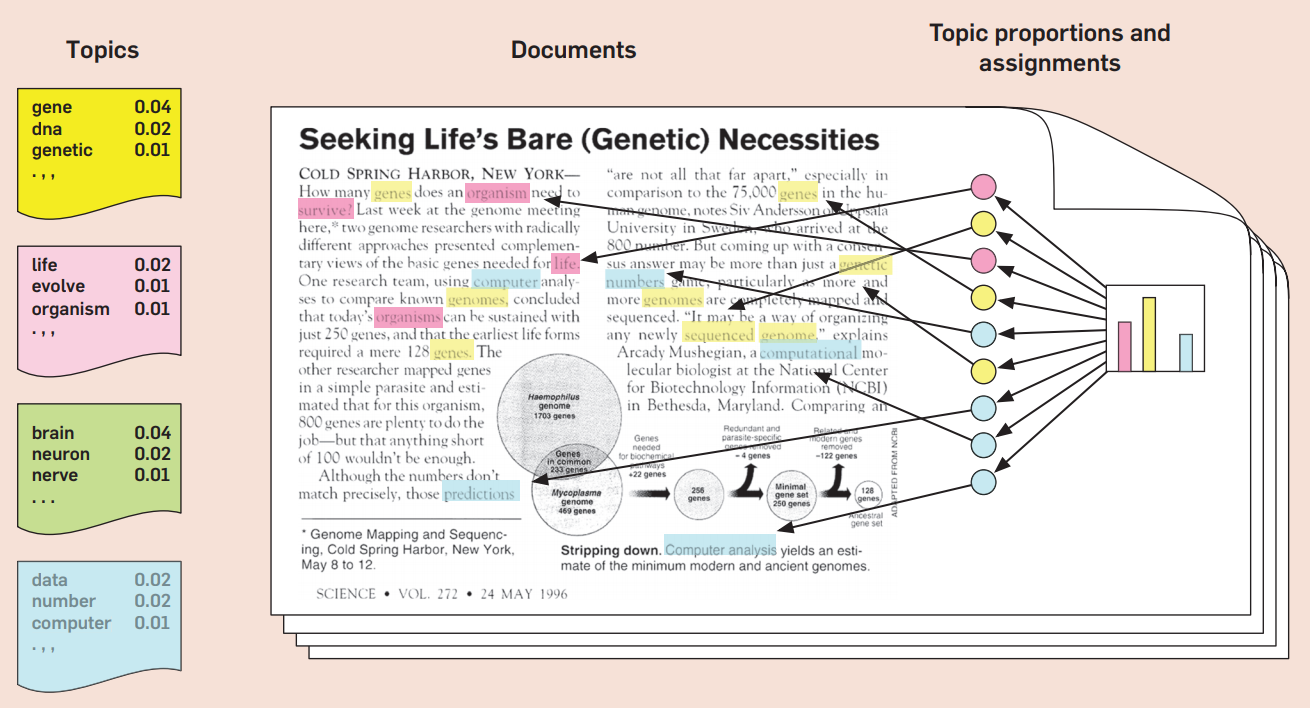
\includegraphics[width=0.8\textwidth]{document/images/lda_topic_model.png}
    % Der Teil in eckigen Klammern ist der Kurztitel für das Table of Contents
    \caption[Schematische Darstellung eines LDA Topic Modelings]{Schematische Darstellung eines LDA Topic Modelings. Quelle: \citetitle{blei_2012} \parencite{blei_2012}}
    \label{fig:lda_example}
\end{figure}

% Wenn wir nicht wollen, dass ein Kapitel auf einer neuen Seite startet, nutzen wir das hier:
{\let\clearpage\relax \chapter{Theoriefindung}}

\Blindtext

%% Bibliography

\setstretch{1.0}
\printbibliography[title={Literaturverzeichnis}]

\end{document}